\documentclass[a4paper,10pt,headlines=3.2]{scrartcl}
\usepackage{graphicx}           %Bilder

%\usepackage[T1]{fontenc}        %Umlaute
%\usepackage[latin1]{inputenc}   %Windows
%\usepackage[utf8x]{inputenc}	%Linux
\usepackage{ucs}

\usepackage[ngerman]{babel}     %Deutsche Sprache
\usepackage{amsmath}            %Math. Zeichen
\usepackage{pifont}             %Skalierbare Schriftart
\usepackage{array}
\usepackage{epsfig}             %Erweiterte Grafiken
\usepackage{makeidx}            %Stichwortverzeichnis
\usepackage[pdftex]{color} 

\newcommand{\changefont}[3]{
\fontfamily{#1} \fontseries{#2} \fontshape{#3} \selectfont}

\makeindex

\usepackage[automark]{scrpage2}
\usepackage[nosectionbib]{apacite}               %Zitieren

%\usepackage[colorlinks]{hyperref}%Hyperlinks

\usepackage{lmodern}
\usepackage{scrpage2}           %KOMA-Script
\usepackage{tipa}
\usepackage{qtree}
\usepackage{wasysym}

\usepackage{remreset}			%Fussnoten global
\makeatletter
\@removefromreset{footnote}{chapter}
\makeatother 

\setcounter{tocdepth}{3}

%Kopfzeilen
\pagestyle{scrheadings}         %Seitenstil scrheadings verwenden

%\setlength{\textheight}{24cm}
%\setlength{\textwidth}{16cm}
%\setlength{\topmargin}{-2cm}
%\setlength{\oddsidemargin}{0cm}

% Groesse des Textbereiches in der Seite
\setlength{\textwidth}{16cm}
\setlength{\textheight}{22cm}
% Kopf- und Fusszeile, Hoehe und Abstand vom Text
\setlength{\headheight}{15pt}
\setlength{\headsep}{0.8cm}
% Linker Seiteneinzug
\setlength{\oddsidemargin}{2.5cm} \addtolength{\oddsidemargin}{-1in}
\setlength{\evensidemargin}{2.5cm} \addtolength{\evensidemargin}{-1in}
% Andere Groessen ausrechnen (vertikal zentrieren)
\setlength{\footskip}{\headsep}
\addtolength{\footskip}{\headheight}
\setlength{\topmargin}{\paperheight}
\addtolength{\topmargin}{-\textheight}
\addtolength{\topmargin}{-\headheight}
\addtolength{\topmargin}{-\headsep}
\addtolength{\topmargin}{-\footskip}
\addtolength{\topmargin}{-2in}
\addtolength{\topmargin}{-0.5\topmargin}

%Abstand zur�cksetzen
\setlength{\headheight}{20pt}

\usepackage{listings} 
\lstset{numbers=left, numberstyle=\tiny, numbersep=5pt} \lstset{language=Java} 
\changefont{cmss}{m}{n}

\clearscrheadfoot
%\renewcommand{\headheight}{40pt} 
\ihead[]{Datenbanken \\Fr�hlingssemester 2011 \\Institut f�r angewandte
Mathematik} % - linke Kopfzeile 
\ohead[asdasd]{�bung 9, Abgabe 3. Mai 2011 \\Adrianus Kleemans
[07-111-693]\\Pinar Kayalar [10-123-453]} % - linke Kopfzeile 
\setheadsepline{.4pt} %Separate Linie im Kopf
\cfoot[\pagemark]{\pagemark} %- mittlere Fusszeile

\begin{document}
\section*{Aufgabe 1}
\begin{figure}[ht]
\centering
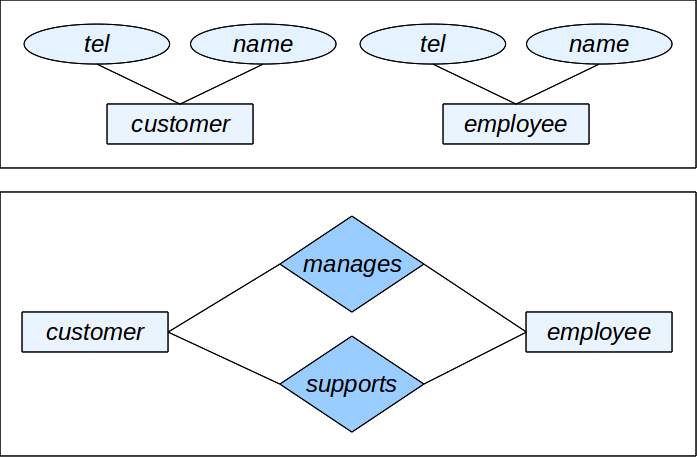
\includegraphics[height=6cm]{aufg1}
\caption{Oben wird Eigenschaft 1 verletzt (zwei Entit�ten mit gleichen Attributen), unten Eigenschaft 2 (zwei Entit�ten haben mehrere  Relationships)}
\end{figure}

\section*{Aufgabe 2}
\begin{figure}[ht]
\centering
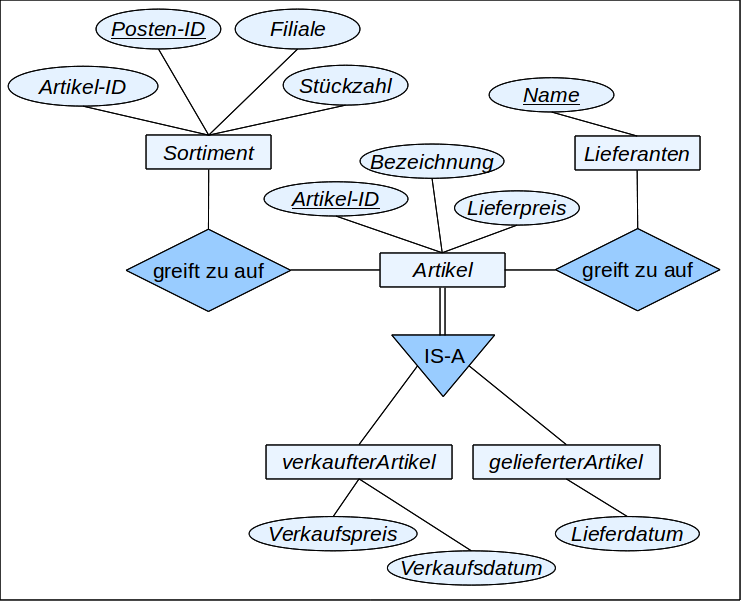
\includegraphics[height=8cm]{aufg2}
\caption{Lagerverwaltung}
\end{figure}
\newpage

\section*{Aufgabe 3}
\begin{figure}[!h]
\centering
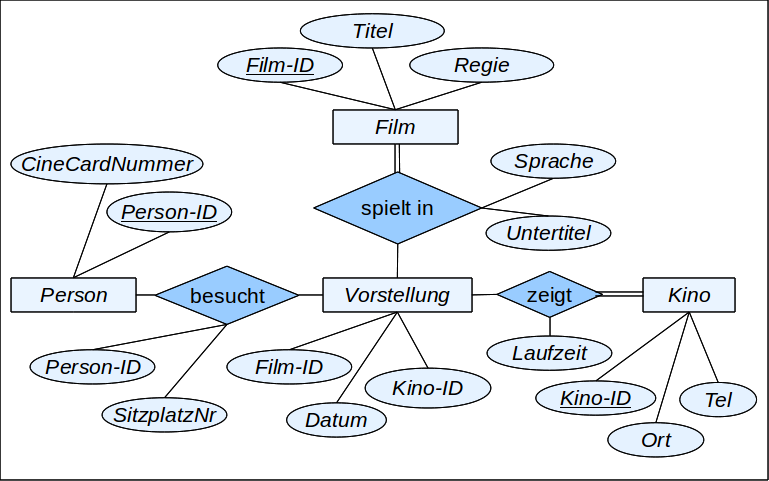
\includegraphics[height=8cm]{aufg3}
\caption{Kinoverwaltung}
\end{figure}

\section*{Aufgabe 4}
\begin{itemize}
 \item[a] Schl�sselkandidaten: (keine, eigener Prim�rschl�ssel n�tig, z.B. borrower\_id)
 \item[b] Schl�sselkandidaten: loan\_number, customer\_id \& loan\_number 
 \item[c] Schl�sselkandidaten: customer\_id, customer\_id \& loan\_number 
 \item[d] Schl�sselkandidaten: customer\_id, loan\_number, customer\_id \& loan\_number
\end{itemize}

\section*{Aufgabe 5}
\begin{figure}[ht]
\centering
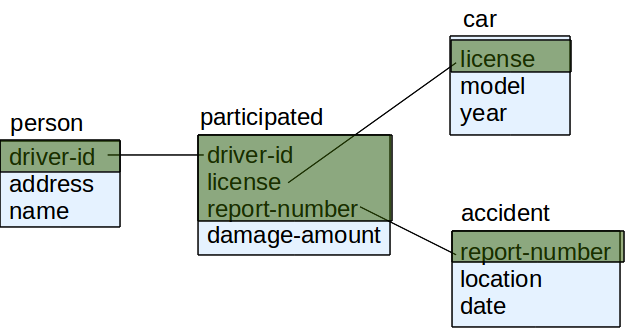
\includegraphics[height=4cm]{aufg5}
\caption{Datenbankschema Autounf�lle}

\end{figure}

\end{document}